\documentclass[a4paper,12pt,twoside,openany]{report}
%
% Wzorzec pracy dyplomowej
% J. Starzynski (jstar@iem.pw.edu.pl) na podstawie pracy dyplomowej
% mgr. inż. Błażeja Wincenciaka
% Wersja 0.1 - 8 października 2016
%
\usepackage{polski}
\usepackage{helvet}
\usepackage[T1]{fontenc}
\usepackage{anyfontsize}
\usepackage[utf8]{inputenc}
\usepackage[pdftex]{graphicx}
\usepackage{tabularx}
\usepackage{array}
\usepackage[polish]{babel}
\usepackage{subfigure}
\usepackage{amsfonts}
\usepackage{verbatim}
\usepackage{indentfirst}
\usepackage[pdftex]{hyperref}
\usepackage{listings}
\lstset{language=Java}  


% rozmaite polecenia pomocnicze
% gdzie rysunki?
\newcommand{\ImgPath}{.}

% oznaczenie rzeczy do zrobienia/poprawienia
\newcommand{\TODO}{\textbf{TODO}}


% wyroznienie slow kluczowych
\newcommand{\tech}{\texttt}

% na oprawe (1.0cm - 0.7cm)*2 = 0.6cm
% na oprawe (1.1cm - 0.7cm)*2 = 0.8cm
%  oddsidemargin lewy margines na nieparzystych stronach
% evensidemargin lewy margines na parzystych stronach
\def\oprawa{1.05cm}
\addtolength{\oddsidemargin}{\oprawa}
\addtolength{\evensidemargin}{-\oprawa}

% table span multirows
\usepackage{multirow}
\usepackage{enumitem}	% enumitem.pdf
\setlist{listparindent=\parindent, parsep=\parskip} % potrzebuje enumitem

%%%%%%%%%%%%%%% Dodatkowe Pakiety %%%%%%%%%%%%%%%%%
\usepackage{prmag2017}   % definiuje komendy opieku,nrindeksu, rodzaj pracy, ...


%%%%%%%%%%%%%%% Strona Tytułowa %%%%%%%%%%%%%%%%%
% To trzeba wypelnic swoimi danymi
\title{Implementacja portalu do grywalizacji z użyciem platformy SPRING i bazy danych Oracle}

% autor
\author{Jacek Kozieja}
\nrindeksu{261053}

% jeśli wykonawca jest tylko jeden, to usuwamy poniższe polecenia


\opiekun{dr inż. Jacek Korytkowski}
 % opcjonalnie
\terminwykonania{16 maja 2017} % data na oświadczeniu o samodzielności
\rok{2017}


% Podziekowanie - opcjonalne
\podziekowania{\noindent
{\Large Podziękowania}
\bigskip

Dziękujemy bardzo serdecznie wszystkim, a w szczególności Rodzinom i~Unii Europejskiej...

\bigskip

{\raggedleft
Zdolny Student i Pracowity Kolega

}

}

% To sa domyslne wartosci
% - mozna je zmienic, jesli praca jest pisana gdzie indziej niz w ZETiIS
% - mozna je wyrzucic jesli praca jest pisana w ZETiIS
%\miasto{Warszawa}
%\uczelnia{POLITECHNIKA WARSZAWSKA}
%\wydzial{WYDZIAŁ ELEKTRYCZNY}
%\instytut{INSTYTUT ELEKTROTECHNIKI TEORETYCZNEJ\linebreak[1] I~SYSTEMÓW INFORMACYJNO-POMIAROWYCH}
% \zaklad{ZAKŁAD ELEKTROTECHNIKI TEORETYCZNEJ\linebreak[1] I~INFORMATYKI STOSOWANEJ}
%\kierunekstudiow{INFORMATYKA}

% domyslnie praca jest inzynierska, ale po odkomentowaniu ponizszej linii zrobi sie magisterska
%\pracamagisterska
%%% koniec od P.W

\opinie{%
  \newpage
\begin{center}
 {\large\bf  Opinia} \\
o pracy dyplomowej magisterskiej wykonanej przez dyplomanta\\
{\bf Zdolnego Studenta i Pracowitego Kolegę} \\
 Wydział Elektryczny, kierunek Informatyka,  Politechnika Warszawska\\
Temat pracy\\
\textit{\bf
TYTUŁ PRACY DYPLOMOWEJ
}\\
\end{center}
\medskip
\noindent
Promotor: {\bf dr inż. Miły Opiekun}\\
Ocena pracy dyplomowej: {\bf bardzo dobry}

\medskip

\centerline{\bf Treść opinii}
   Celem pracy dyplomowej panów dolnego Studenta i Pracowitego Kolegi  było
opracowanie systemu pozwalającego symulować  i opartego o oprogramowanie o
otwartych źródłach (ang. Open Source). Jak piszą Dyplomanci, starali się opracować
system, który łatwo będzie dostosować do zmieniających się dynamicznie wymagań,
będzie miał niewielkie wymagania sprzętowe i umożliwiał dalszą łatwą rozbudowę oraz
dostosowanie go do potrzeb.
Przedstawiona do recenzji praca składa się z krótkiego wstępu jasno i
wyczerpująco opisującego oraz uzasadniającego cel pracy, trzech rozdziałów (2-4)
zawierających opis istniejących podobnych
rozwiązań, komponentów rozpatrywanychjako kandydaci do
tworzonego systemu i wreszcie zagadnień wydajności wirtualnych
rozwiązań. Piąty rozdział to opis przygotowanego przez
Dyplomantów środowiska obejmujący opis konfiguracji
środowiska oraz przykładowe ćwiczenia laboratoryjne. Ostatni
rozdział pracy to opis możliwości dalszego
rozwoju projektu. W ramach przygotowania pracy Dyplomanci zebrali i przedstawili w
bardzo przejrzysty sposób duży zasób informacji, co świadczy o dobrej orientacji
w nowoczesnej i ciągle intensywnie rozwijanej tematyce stanowiącej
zakres pracy i o umiejętności przejrzystego przedstawienia tych
wyników. Praca zawiera dwa dodatki, z których pierwszy obejmuje wyniki
eksperymentów i badań nad wydajnością, a drugi to źródła
skryptów budujących środowisko.

 Dyplomanci dość
dobrze zrealizowali postawione przed nimi zadanie,
wykazali się więc umiejętnością zastosowania w praktyce wiedzy
przedstawionej w rozdziałach 2-4.  Uważam, że cele postawione w założeniach pracy zostały pomyślnie
zrealizowane. Proponuję ocenę bardzo dobrą (5).

\vskip 1cm
{
\raggedleft
(data, podpis)\kern1cm

}
  \newpage
  \newpage
\begin{center}
 {\large\bf  Recenzja } \\
pracy dyplomowej magisterskiej wykonanej przez dyplomanta\\
{\bf Zdolnego Studenta i Pracowitego Kolegę} \\
 Wydział Elektryczny, kierunek Informatyka,  Politechnika Warszawska\\
Temat pracy\\
\textit{\bf
TYTUŁ PRACY DYPLOMOWEJ
}\\
\end{center}
\medskip
\noindent
Recenzent: {\bf prof. nzw. dr hab. inż. Jan Surowy}\\
Ocena pracy dyplomowej: {\bf bardzo dobry}
\medskip


\centerline{\bf Treść recenzji}
   Celem pracy dyplomowej panów dolnego Studenta i Pracowitego Kolegi  było
opracowanie systemu pozwalającego symulować  i opartego o oprogramowanie o
otwartych źródłach (ang. Open Source). Jak piszą Dyplomanci, starali się opracować
system, który łatwo będzie dostosować do zmieniających się dynamicznie wymagań,
będzie miał niewielkie wymagania sprzętowe i umożliwiał dalszą łatwą rozbudowę oraz
dostosowanie go do potrzeb.
Przedstawiona do recenzji praca składa się z krótkiego wstępu jasno i
wyczerpująco opisującego oraz uzasadniającego cel pracy, trzech rozdziałów (2-4)
zawierających bardzo solidny i przejrzysty opis: istniejących podobnych
rozwiązań (rozdz. 2), komponentów rozpatrywanychjako kandydaci do
tworzonego systemu (rozdz. 3) i wreszcie zagadnień wydajności wirtualnych
rozwiązań, zwłaszcza w kontekście współpracy  kilku elementów
 sieci (rozdział 4). Piąty rozdział to opis przygotowanego przez
Dyplomantów środowiska obejmujący opis konfiguracji
środowiska oraz przykładowe ćwiczenia laboratoryjne (5 ćwiczeń). Ostatni, szósty
rozdział pracy to krótkie zakończenie, które wylicza także możliwości dalszego
rozwoju projektu. W ramach przygotowania pracy Dyplomanci zebrali i przedstawili w
bardzo przejrzysty sposób duży zasób informacji o narzędziach, Rozdziały 2, 3 i 4 świadczą o dobrej orientacji
w nowoczesnej i ciągle intensywnie rozwijanej tematyce stanowiącej
zakres pracy i o umiejętności syntetycznego, przejrzystego przedstawienia tych
wyników. Drobne  mankamenty tej części pracy to zbyt skrótowe omawianie
niektórych zagadnień technicznych, zakładające dużą początkową wiedzę czytelnika
i dość niestaranne podejście do powołań na źródła.
Utrudnia to w pewnym stopniu czytanie pracy i zmniejsza jej wartość dydaktyczną
(a ta zdaje się być jednym z celów Autorów), ale jest zrekompensowane zawartością
merytoryczną. Praca zawiera dwa dodatki, z których pierwszy obejmuje wyniki
eksperymentów i badań nad wydajnością, a drugi to źródła
skryptów budujących środowisko. Praca
zawiera niestety dość dużą liczbę drobnych błędów redakcyjnych, ale nie wpływają
one w sposób istotny na na jej czytelność i wartość. W całej pracy przewijają
się samodzielne, zdecydowane wnioski Autorów, które są wynikiem własnych i
oryginalnych badań.  Rozdział 5 i dodatki pracy przekonują mnie, że Dyplomanci dość
dobrze zrealizowali postawione przed nimi zadanie. Pozwala to stwierdzić, że
wykazali się więc także umiejętnością zastosowania w praktyce wiedzy
przedstawionej w rozdziałach 2-4. Kończący pracę rozdział szósty świadczy o
dużym (ale moim zdaniem uzasadnionym) poczuciu własnej wartości i jest
świadectwem własnego, oryginalnego spojrzenia na tematykę przedstawioną w pracy
dyplomowej. Uważam, że cele postawione w założeniach pracy zostały pomyślnie
zrealizowane. Proponuję ocenę bardzo dobrą (5).

\vskip 1cm
{
\raggedleft
(data, podpis)\kern1cm

}
}

\streszczenia{
  \newpage
\begin{center}
\large \bf
Implementacja portalu do grywalizacji z użyciem platformy SPRING i bazy danych Oracle
\end{center}

\section*{Streszczenie}
Praca składa się z krótkiego wstępu opisującego cel oraz strukturę wykonanego projektu, trzech rozdziałów
zawierających opis wykorzystanych technologii (szkielet Angular, szkielet Spring i baza danych Oracle) i przykłady ich zastosowań w projekcie. Czwarty rozdział to opis zagadnień związanych z bezpieczeństwem współczesnych aplikacji internetowych. Rozdział piąty przedstawia wdrożenie aplikacji do chmury obliczeniowej. W rozdziale szóstym można zapoznać się z działaniem aplikacji w praktyce - zawiera on opis funkcjonalności z perspektywy Użytkownika końcowego. Ostatni rozdział to wnioski, dotyczące wydajności i sposobów tworzenia aplikacji.

\bigskip
{\noindent\bf Słowa kluczowe:} Spring, Angular, Oracle

\vskip 2cm


\begin{center}
\large \bf
Implementation of gamification web portal based on SPRING framework and Oracle databse
\end{center}

\section*{Abstract}
This thesis consists of a short introduction that describes goal and structure of a project. Next three chapters depict used technologies (Angular framework, Spring framework and Oracle database) and their use in the project. Fourth chapter is a description of security topics related to modern web applications. Fifth chapter shows cloud migration of a system. The sixth chapter includes description of funcionalities from an end-user perspective - it shows a practical use of the application. The last one is a conclusion about overall performance and approach to application development.

\bigskip
{\noindent\bf Keywords:} Spring, Angular, Oracle

\vfill
}

\begin{document}
\maketitle

%-----------------
% Wstęp
%-----------------
\chapter{Wstęp}
\section{Grywalizacja}
	Grywalizacja, gryfikacja lub gamifikacja, to zgodnie z definicją [Wikipedia] "Wykorzystanie mechaniki znanej np. z gier fabularnych i komputerowych, do modyfikowania zachowań ludzi w sytuacjach niebędących grami, w celu zwiększenia zaangażowania ludzi." Ta szeroka definicja obejmuje rozwiązania stosowane w marketingu, zarządzaniu projektami jak i edukacji. Założeniem stworzonej aplikacji jest motywowanie grup ludzi do wspólnej pracy poprzez system wyzwań i nagród. Należy jednak pamiętać że o ile aplikacja pomaga zarządzać zadaniami, prowadzić ranking i kontrolować rozwój użytkowników, o tyle weryfikacja wykonanych zadań czy przyznawanie fizycznych nagród pozostaje obowiązkiem administratora. Stworzone rozwiązanie było także pretekstem do zbadania współczesnych technologii wytwarzania aplikacji internetowych, opisanych w dalszej części pracy. 
	\section{Projekt}
	Ideę działania aplikacji przybliżyć mogą poniższe przykładowe Przypadki Użycia:\\
	UC Użytkownika:\\
	Wykonanie Zadania
	\begin{enumerate}
		\item Użytkownik loguje się do Systemu.
		\item Użytkownik wybiera opcję ,,Wykonaj Zadanie'' -> (lub skanuje QR)
		\item System wyświetla formularz wykonania Zadania.
		\item Użytkownik wpisuje numer Zadania.
		\item System dodaje zadanie i punkty Użytkownikowi
	\end{enumerate}
	Przejrzenie tabeli Rankingu
	\begin{enumerate}
		\item Użytkownik loguje się do Systemu.
		\item Użytkownik wybiera opcję ,,Ranking''.
		\item System wyświetla tabelę Użytkowników.
		\item Użytkownik wybiera sortowanie malejąco, po Punktach.
		\item System wyświela posortowaną listę.
	\end{enumerate}
	UC Administratora:\\
	Dodanie nowego Zadania
	\begin{enumerate}
		\item Administrator loguje się do systemu
		\item Administrator wybiera opcję ,,Dodaj Zadanie''
		\item System wyświetla formularz dodania Zadania.
		\item Administrator podaje opis, datę końcową i punkty Zadania.
		\item System generuje numer Zadania i zapisuje je.
	\end{enumerate}
	Przynanie Odznaki Użytkownikom
	\begin{enumerate}
		\item Administrator loguje się do Systemu.
		\item Administrator wybiera opcję ,,Odznaki''.
		\item System wyświetla okno edycji Odznak.
		\item Administrator wybiera opcję ,,Przyznaj odznakę''
		\item System wybiera okno wyboru odznaki.
		\item Administrator wybiera Odznakę.
		\item System wyświetla okno wyboru Użytkowników.
		\item Administrator wybiera UżytkownikóW.
		\item System przyznaje odznakę wybranym Użytkownikom.
	\end{enumerate}
	
	(Jak starczy czasu na koniec to może też diagram UC)
	Poniższe diagramy klas przedstawiają strukturę modułu GLogin - oddzielnie dla wnętrza (,,back-end'') i fasady (,,front-end''). Są one reprezentatywne dla całości projektu, zaś stworzenie pełnej dokumentacji uważam za odpowiedni temat dla oddzielnej pracy dyplomowej. Prywatne zmienne posiadające publiczne metody dostępowe zostały przedstawione jako zmienne publiczne. Redukuje to liczbę metod i zwiększa czytelność diagramów.
	\begin{figure}[!htbp]
		\begin{center}
			\centering
			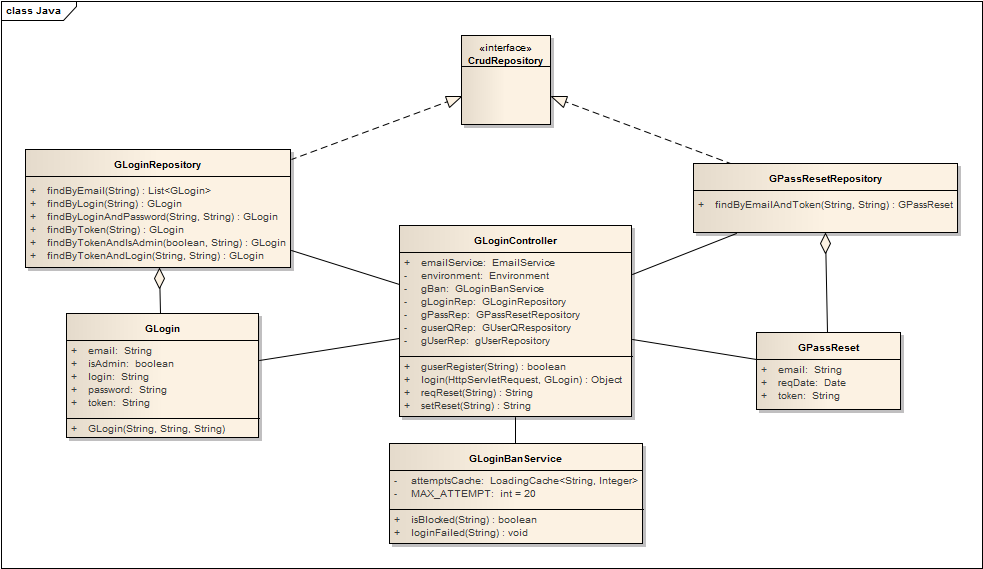
\includegraphics[width=\textwidth]{\ImgPath/rys/UML-Java.png}
		\end{center}
		\caption{Diagram klas w języku Java.}
		\label{UMLJava}
	\end{figure}
		\begin{figure}[!htbp]
			\begin{center}
				\centering
				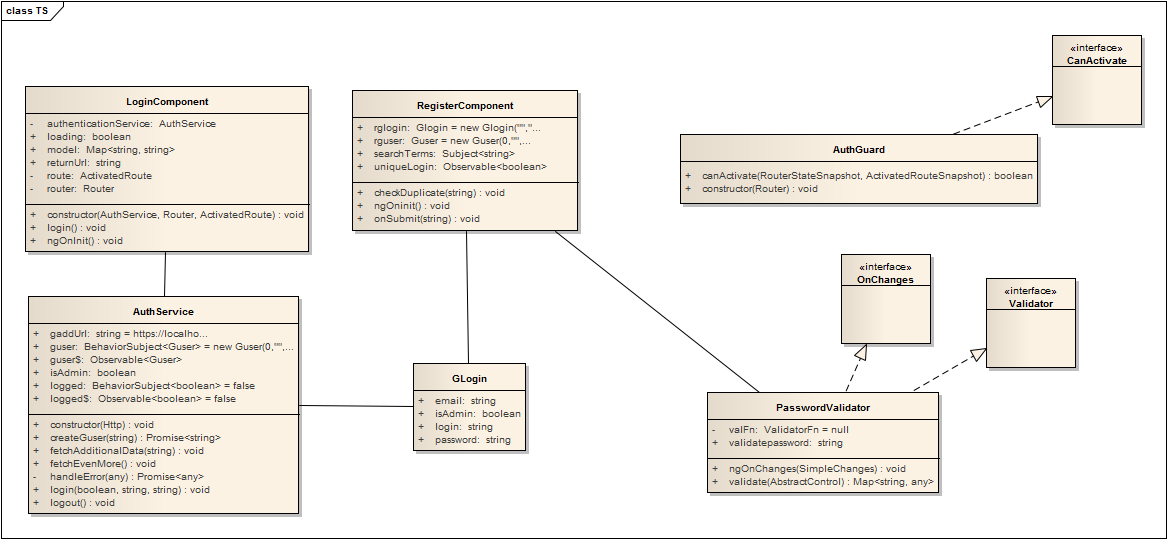
\includegraphics[width=\textwidth]{\ImgPath/rys/UML-TS.png}
			\end{center}
			\caption{Diagram klas w języku TypeScript.}
			\label{UMLTS}
		\end{figure}
\section{Użyte technologie}
Do wykonania aplikacji użyto poniższych technologii: 
	\begin{figure}[!htbp]
		\begin{center}
			\centering
			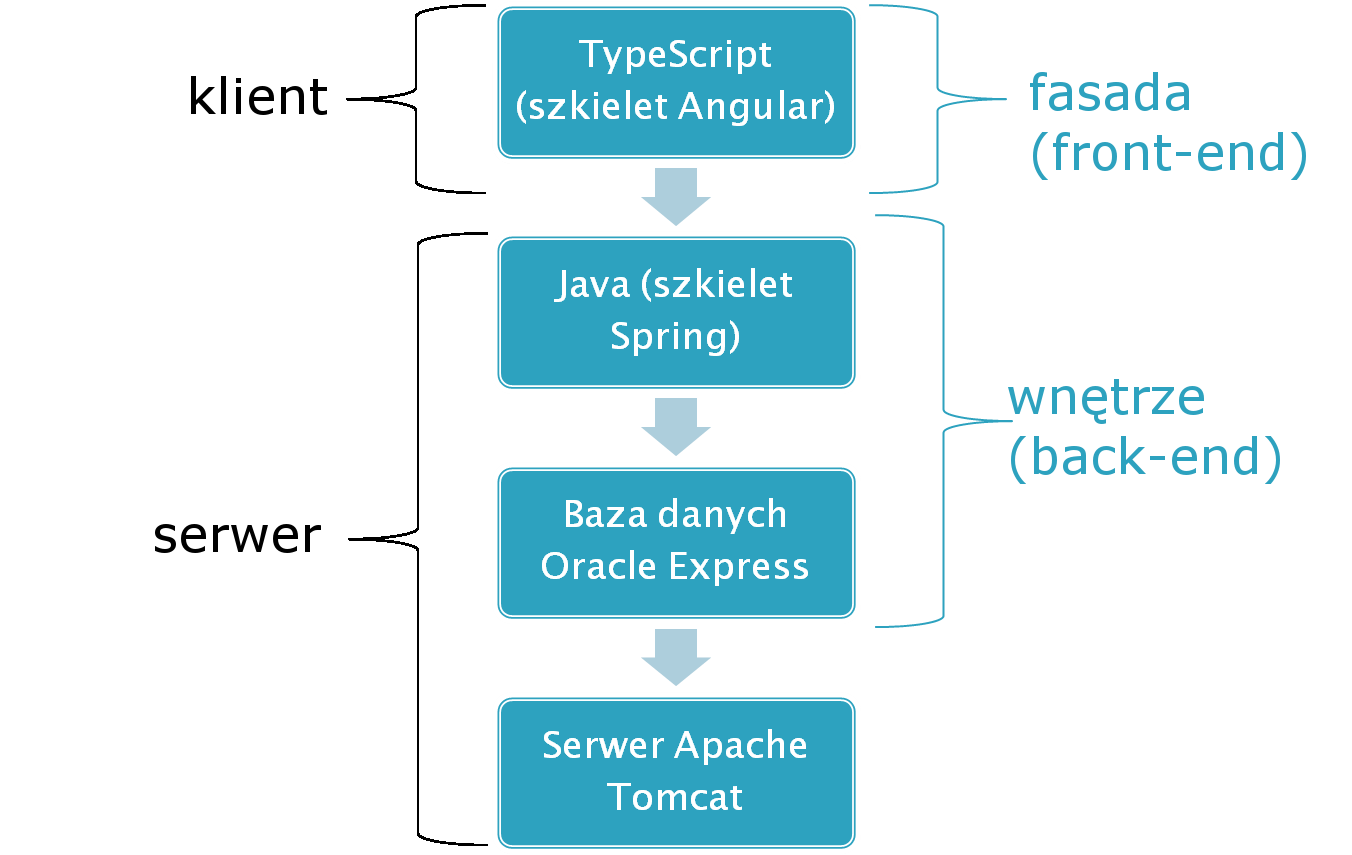
\includegraphics[width=\textwidth]{\ImgPath/rys/technologies.png}
		\end{center}
		\caption{Języki, szkielety i systemy bedące częścią projektu.}
		\label{technologies}
	\end{figure}	
\section{Wzorzec MVC}
- o wzorcu MVC ogólnie + mądry rysunek\\
MVC to wzorzec architektoniczny służący do organizowania struktury systemów interaktywnych. Składa się on z trzech części:
	\begin{enumerate}
		\item Model - reprezentuje dane i wykonuje logikę biznesową.
		\item Widok - wyświetla dane pobrane z Modelu.
		\item Kontroler - reaguje na dane wejściowe użytkownika. Przesyła żądania wykonania logiki biznesowej do Modelu i zmian Widoku. 
	\end{enumerate}
Zarówno Angular jak i Spring samodzielnie realizują wzorzec MVC. Jednak gdy połączymy te dwie technologie, sytuacja zmienia się. Warstwa kontrolera przeniesiona jest do Angulara i jest wykonywana przez przeglądarkę. To samo samo dzieje się z warstwą widoku. Po stronie serwerowej Springa pozostaje warstwa modelu. Ten rozdział powoduje że potrzebny jest odpowiedni sposób komunikacji klient-serwer. Nazywa się on REST API. Skróty te oznaczają Representational State Transfer i Application Programming Interface. Pierwszy skrót oznacza bezstanową wymianę tekstowych zasobów sieciowych. Przykładem są tu zapytania HTTP GET, POST, PUT, DELETE. Drugi skrót oznacza jednoznacznie zdefiniowany sposób komunikacji między komponentami. W wypadku aplikacji internetowej oznacza to że strona serwerowa odbierając zapytanie HTTP pod danym adresem, powinna zwrócić odpowiedź w postaci XML lub JSON.
		\begin{figure}[!htbp]
			\begin{center}
				\centering
				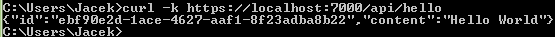
\includegraphics[width=\textwidth]{\ImgPath/rys/testAPI.png}
			\end{center}
			\caption{Zapytanie do API i odpowiedź. Taka komunikacja pozwala wykorzystać tą samą warstwę modelu w kilku różnych aplikacjach.}
			\label{UMLTS}
		\end{figure}
- o tym jakie technologie u mnie realizują którą warstwę. O tym że Angular narzuca sobie warstwę kontrolera i potrzebujemy REST API\\
- Podział na moduły - klient-admin + pakiety do każdej poszczególnej funkcjonalnosci. Przedrostek g podyktowany zbieżnoscią nazw takich jak login czy user z natywnymi elementami użytych platform.

\chapter{Spring}
-framework ogólnego przeznaczenia\\
-Spring boot - co to?\\
- konfiguracja xml vs adnotacje\\
- maven(wklej i omów prosty przykład, napisz że mój jest bardziej pro, no ale)\\
- przydatne moduły Springa - Data, JPA, Security, Jackson\\
- moje REST API - klient\\
- moje REST API - admin\\

\chapter{Baza danych Oracle}
-Krótka historia baz oracla \\
- Konfiguracja bazy w Springu\\
- metody optymalizacji - stronicowanie, te takie priorytety kolumn\\
- PLSQL - SQL na sterydach - porównaj, opisz możliwosci, krótkie zapytania na naszej bazie\\

\chapter{Angular 2}
-cechy charakterystyczne, dlaczego taki modny - standalone, własny serwer, SINGLE-PAGE APP\\
- Typescript vs Javascript - statyczne typowanie, kompatybilnosc z JS i bibliotekami - moja konfiguracja bibliotek i moja konfiguracja kompilowania i wrzucania do projektu Springa\\
- serwisy i modele po stronie angulara\\
- moje kontrolery - klient - w tym opis podstawowych elementóW kontrolera, to że własny css\\
- moje kontrolery - admin\\

\chapter{Bezpieczeństwo}
- token do CSRF\\
- https\\
- token logowania wymieniany za hasło - policz też entropię, ile zajmie złamanie, wykaż że razem z punktem [BAN na IP] strona jest bezpieczna\\
- reset i zmiana hasła\\
- BAN na IP\\
- SQL Injection - nie działa bo Java\\

\chapter{Wdrożenie systemu}
-Tomcat i pliki jar
- Jakie są mniej więcej chmury, konfiguracja i screeny jak wrzucam - TBA
\chapter{Wnioski}
- policz czasy ładowania strony i porównaj z pro stronami - wp, facebook. Dodaj dużo danych i sprawdź w stresie może.\\
-wady debugowania Angulara, czasy kompilacji Springa/Mavena/Tomcata - czy tyle warstw aplikacji na pewno jest nam potrzebne?\\
- Zmiany w technologii - im bliżej frontendu tym szybciej. Warto odpowiedzieć sobie na pytanie - w czym ta nowa technologia jest lepsza od mojej, ale też dobierać technologię do projektu?


\chapter{Schowek}
\label{Schowek}

\section{Rzeczy}
\ref{Schowek}
\cite{Stevens}
\begin{itemize}
	\item Punkt 1
	\item Punkt 2
\end{itemize}
\begin{figure}[!htbp]
	\begin{center}
		\centering
		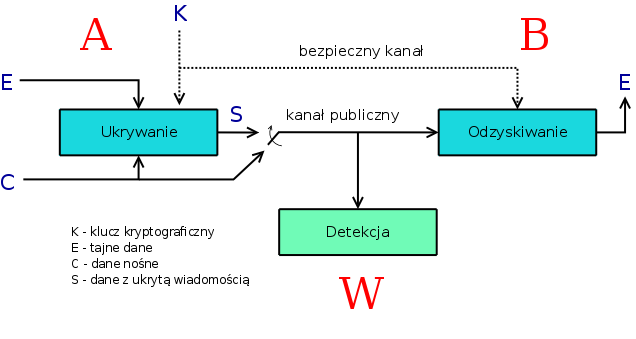
\includegraphics[scale=0.4]{\ImgPath/rys/schemat_komunikacji.png}
	\end{center}
	\caption{Schemat komunikacji steganograficznej}
	\label{schematKomunikacji}
\end{figure}
\begin{lstlisting}
int main(String args){}
\end{lstlisting}


\begin{thebibliography}{99}
\addcontentsline{toc}{chapter}{Bibliografia}
\bibitem{Pierwsza}{Dokumentacja Springa/Mądra książka o Springu}
\bibitem{Druga}{Mądra książka o PLSQL - ta do wersji 10 co czytałes w PKO}
\bibitem{Trzecia}{Dokumentacja Angulara}
\bibitem{Czwarta}{Ta książka o gamifikacji albo wikipedia }
\bibitem{Piąta}{Cos o bezpieczenstwie - poszukaj w materialach do zajęć z bezpieczeństwa, oni ogarniali temat}
\bibitem{Szósta}{Thinking in JAVA?? Jak znajdziesz fragment który się przyda}

\bibitem{Stevens}{W. R. Stevens, G. R. Wright, ,,Biblia TCP/IP tom 1'', RM, 
1998.}

\end{thebibliography}

\zakonczenie  % wklejenie recenzji i opinii

\end{document}
%+++ END +++
